\documentclass[
]{beamer}

\usepackage[czech]{babel}
\usepackage[utf8]{inputenc}
\usepackage[T1]{fontenc}
\usepackage{booktabs}
\usetheme[
  workplace=fi,
]{MU}

% Packages
\usepackage{tikz}

\begin{document}

% TODO: Remove the left part of the footer.
\title{Adaptabilní systém pro výuku programování}
%\subtitle{Obhajoba diplomové práce}
\author[T.\,Effenberger]{Tomáš Effenberger} %\\ 410350@mail.muni.cz}
\institute[FI MU]{Fakulta informatiky Masarykovy univerzity}
\date{\today}
%\subject{Předmět prezentace}
%\keywords{klíčová, slova, prezentace}

\begin{frame}[plain]
\maketitle
\end{frame}

%\begin{frame}{Osnova}
%\tableofcontents
%\end{frame}

% Mozna rozsireni:
% - dalsi analyzy (napr. mereni vykonu)
% - implementace, napr. transformace RoboKodu

\begin{frame}{RoboMise}
% Mise, rozsah, optimalni obtiznost, flow, blokove programovani.
% Existujici systemy (HoC) a pridana hodnota (vyzkum adaptability).
% Stav (2. prototyp), testovani na skolach.
\begin{figure}
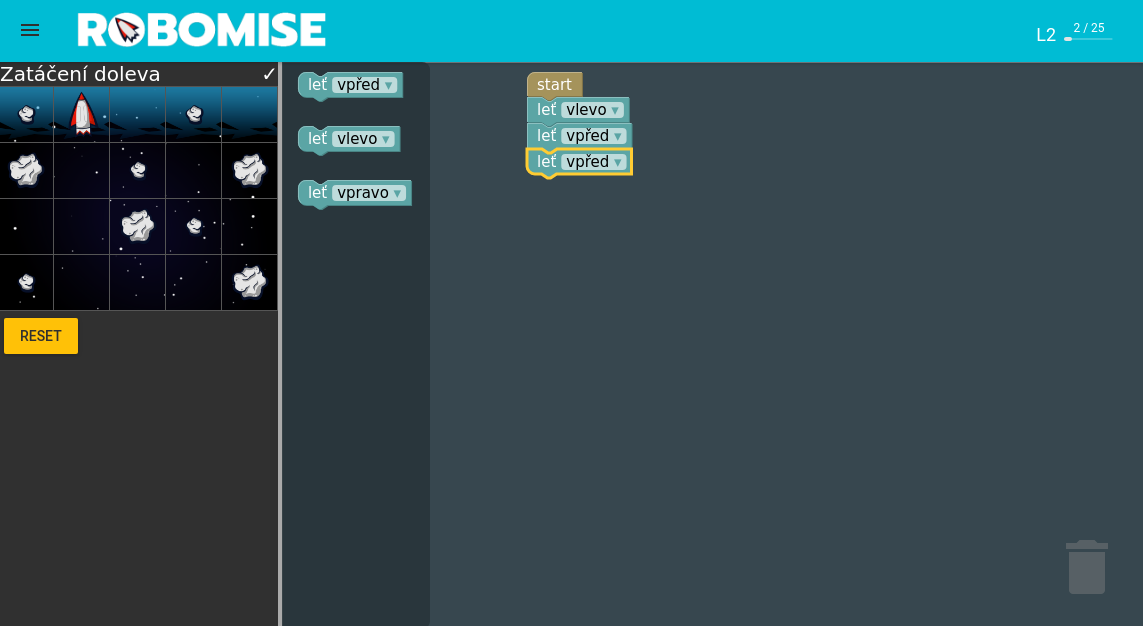
\includegraphics[width=\textwidth,height=.65\textheight,keepaspectratio]{../img/robomission-task1}
\end{figure}
\end{frame}

\begin{frame}{InterSoB}
% Strategie pro podporu motivace a uceni
% -> tak jednoduche, ze to jde zvladnout i poslepou.
\begin{figure}
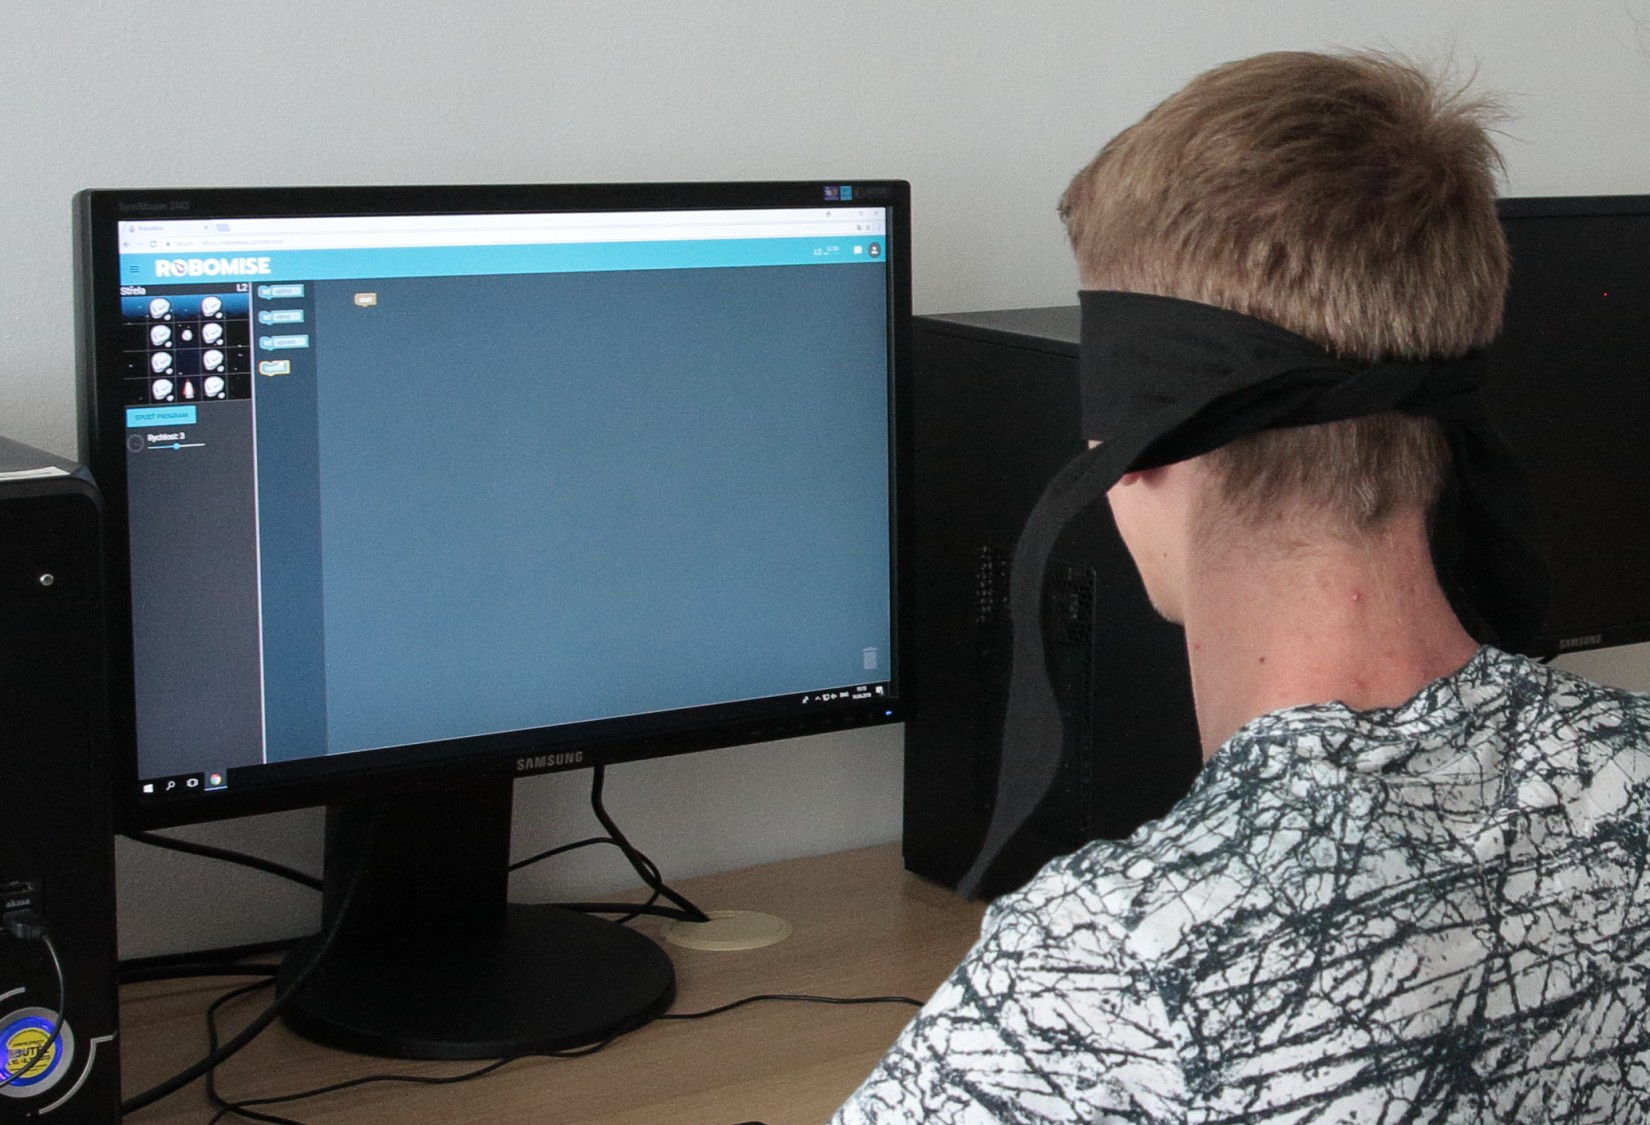
\includegraphics[width=\textwidth,height=.75\textheight,keepaspectratio]{../img/intersob}
\end{figure}
\end{frame}

\begin{frame}{Herní svět}
% Navrh programovací hry: musi bavit a umoznovat rozpeti obtiznosti.
% robot na mrizce, staly let vpred, vice zakladnich akci.
% Herni prvky: diamanty, asteroidy, meteorodiy, cervi diry, barvy.
% Zduraznit inovaci oproti znamym hram ve stalem letu vpred.
\begin{figure}
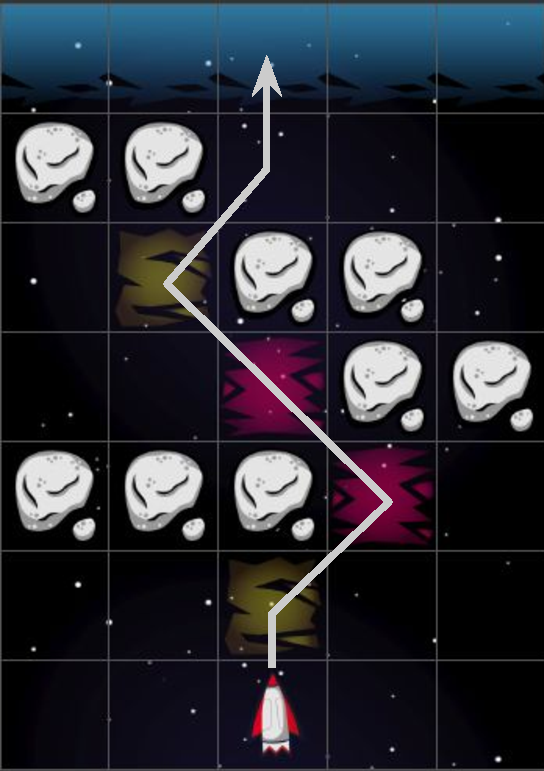
\includegraphics[width=\textwidth,height=.65\textheight,keepaspectratio]{../img/spaceworld-path}
%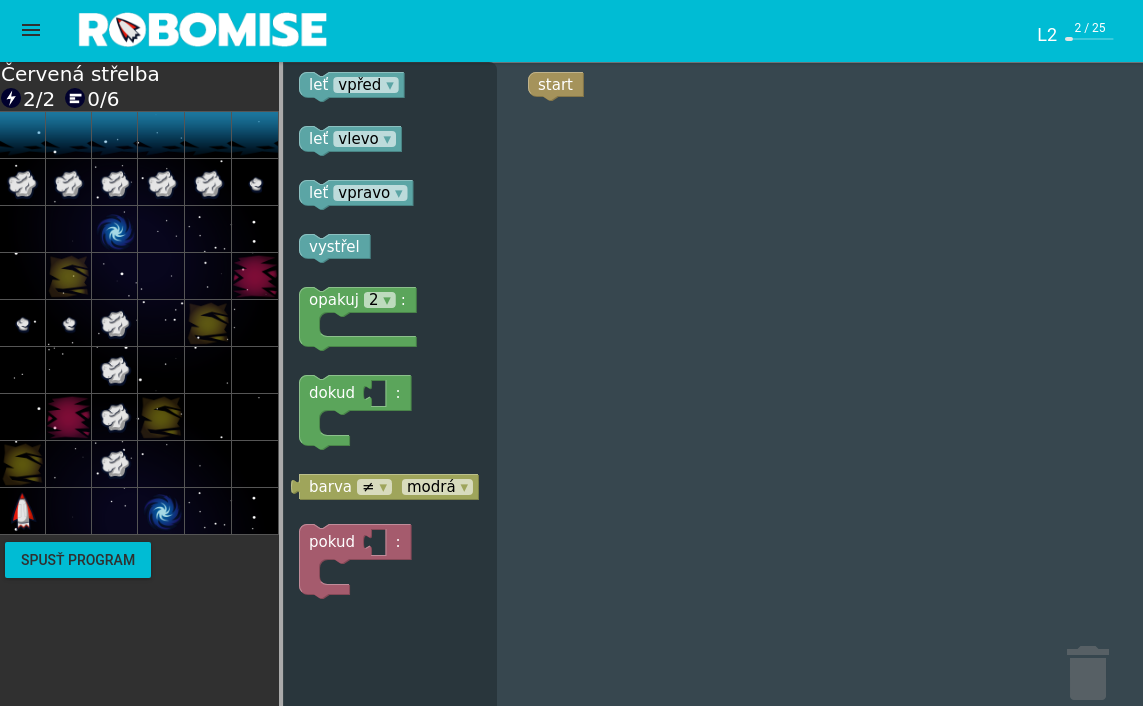
\includegraphics[width=\textwidth,height=.65\textheight,keepaspectratio]{../img/robomission-task3}
\end{figure}
\end{frame}


\begin{frame}{Programovací bloky}
% Proc: odstraneni problemu se syntaxi.
% Bloky: prikazy, cykly, podminky; kontrola barev a pozice.
\begin{figure}
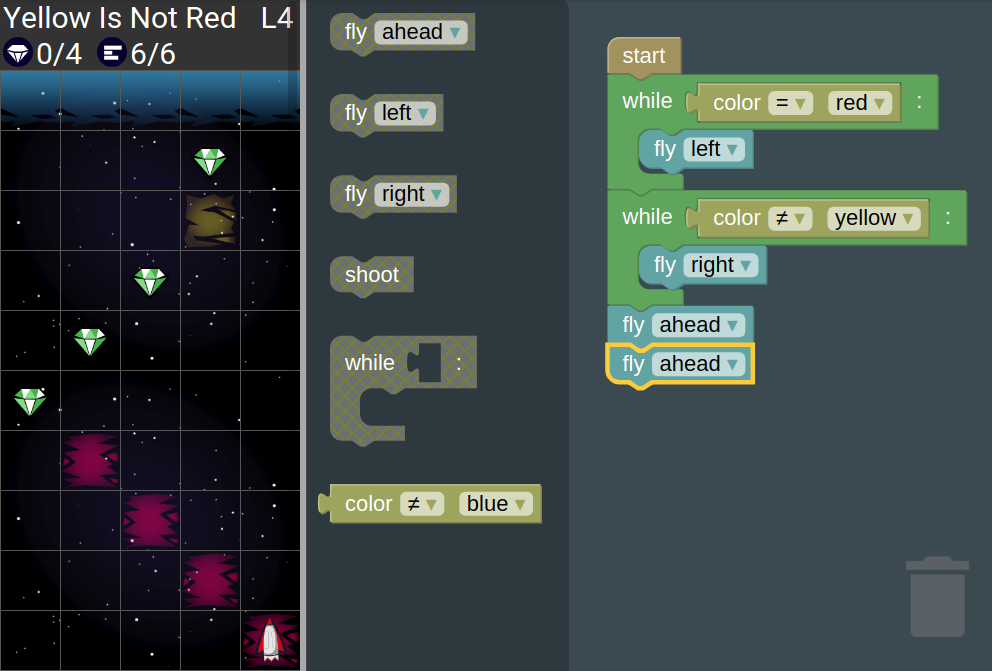
\includegraphics[width=\textwidth,height=.65\textheight,keepaspectratio]{../img/robomission-yellow-is-not-red-whiles}
%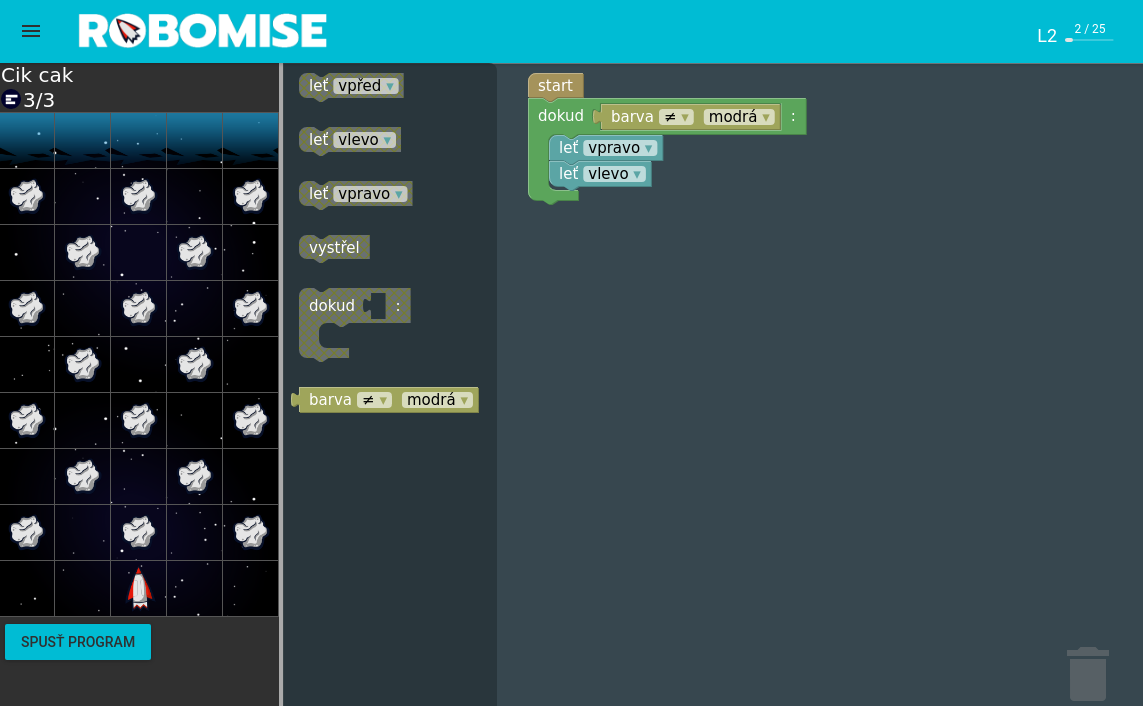
\includegraphics[width=\textwidth,height=.65\textheight,keepaspectratio]{../img/robomission-task2}
\end{figure}
\end{frame}

\begin{frame}{Instrukce a vysvětlení}
% Adaptabilni instrukce a mini-vysvetleni.
\begin{figure}
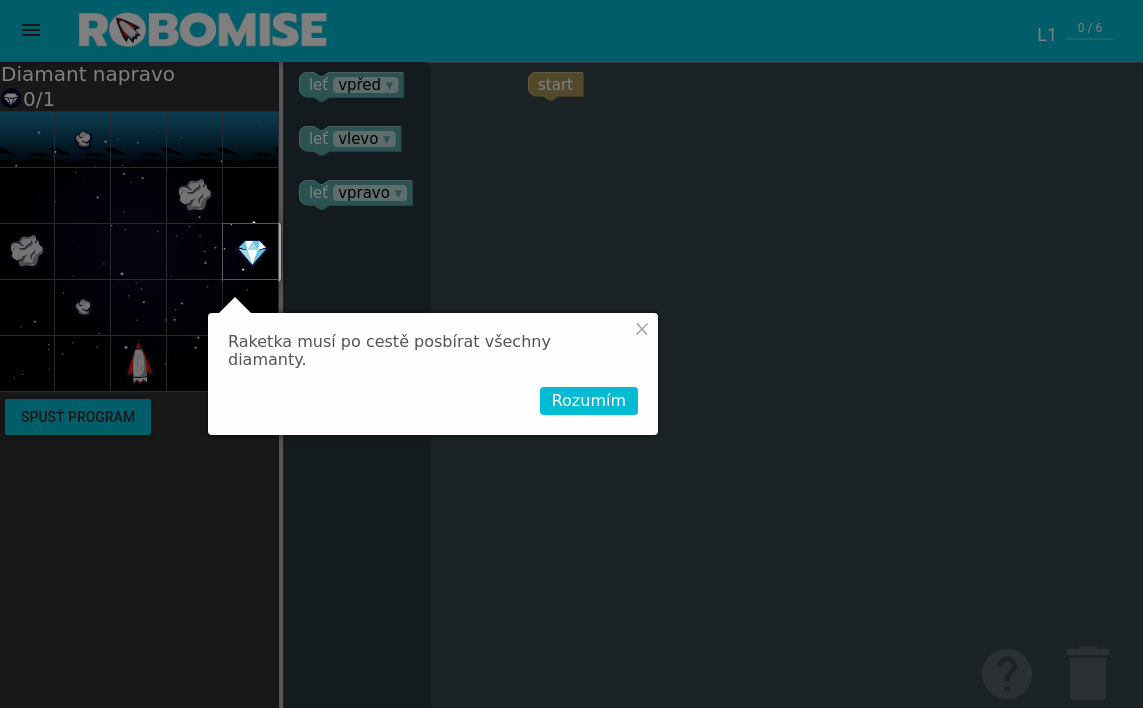
\includegraphics[width=\textwidth,height=.65\textheight,keepaspectratio]{../img/robomission-mini-instruction}
\end{figure}
\end{frame}

\begin{frame}{Levely a kredity}
% Motivacni prvky: kredity, levely.
% Mastery learning.
%\vspace{-10pt}
\begin{figure}
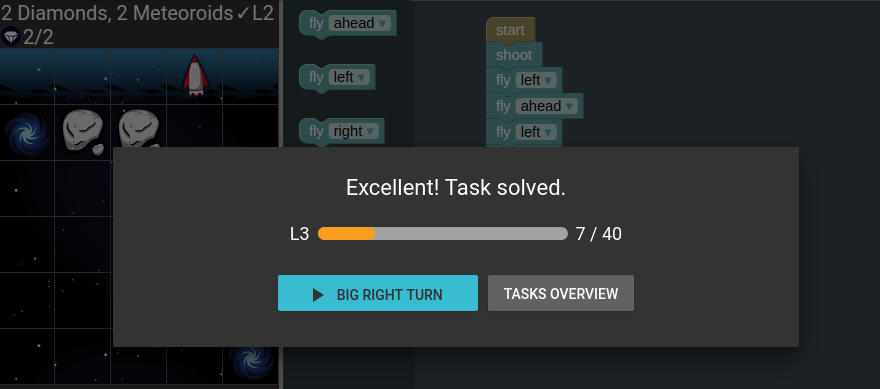
\includegraphics[width=0.9\textwidth,height=.65\textheight,keepaspectratio]{../img/robomission-levels-credits}
\end{figure}
\end{frame}

\begin{frame}{Přehled úloh}
% Pres 80 uloh, rozdelenych do 9 levelu, kazdy level do 3 fazi.
\begin{figure}
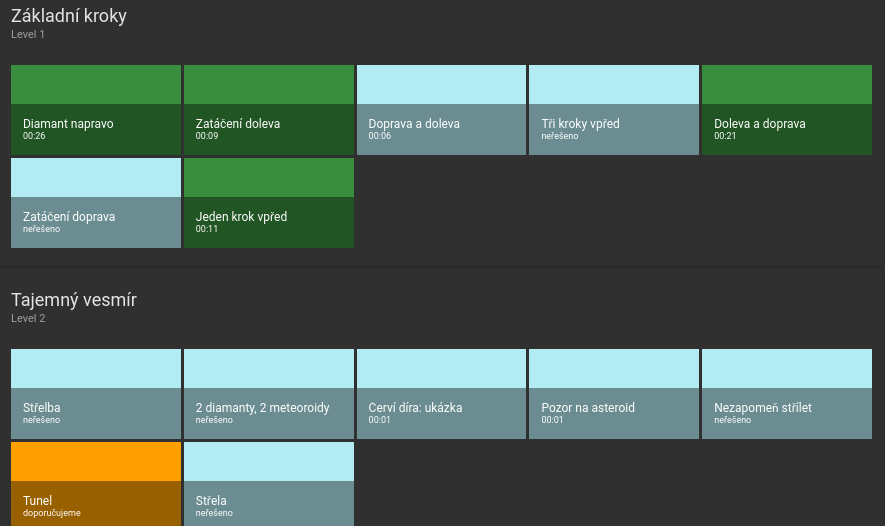
\includegraphics[width=\textwidth,height=.75\textheight,keepaspectratio]{../img/robomission-tasks-overview}
\end{figure}
\end{frame}

\begin{frame}{Anglická lokalizace}
\begin{figure}
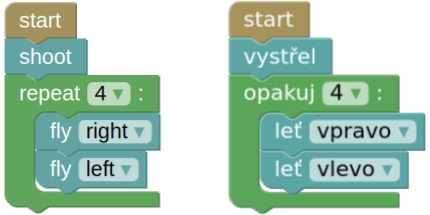
\includegraphics[width=0.5\textwidth,height=.75\textheight,keepaspectratio]{../img/roboblocks-english-czech}
\end{figure}
\end{frame}


\begin{frame}{Editor úloh}
% Online editor úloh. Moznost psat reseni v Pythonu a editovat mrizku ve vimu.
% Textovy format (markdown).
\begin{figure}
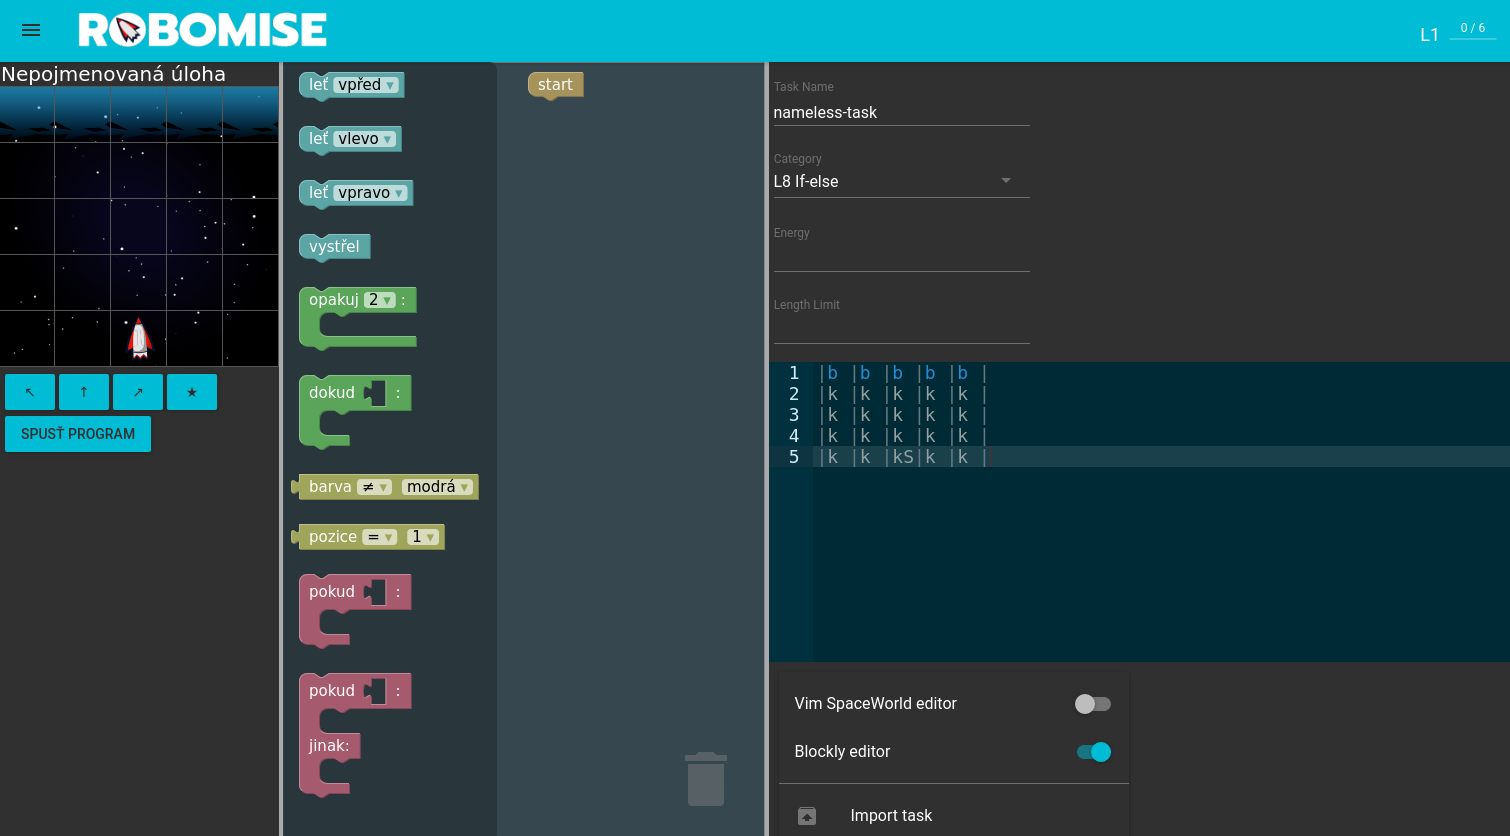
\includegraphics[width=\textwidth,height=.75\textheight,keepaspectratio]{../img/task-editor}
\end{figure}
\end{frame}


\begin{frame}{Model domény}
% Pres 80 uloh, rozdelenych do 9 levelu, kazdy level do 3 fazi.
\begin{figure}
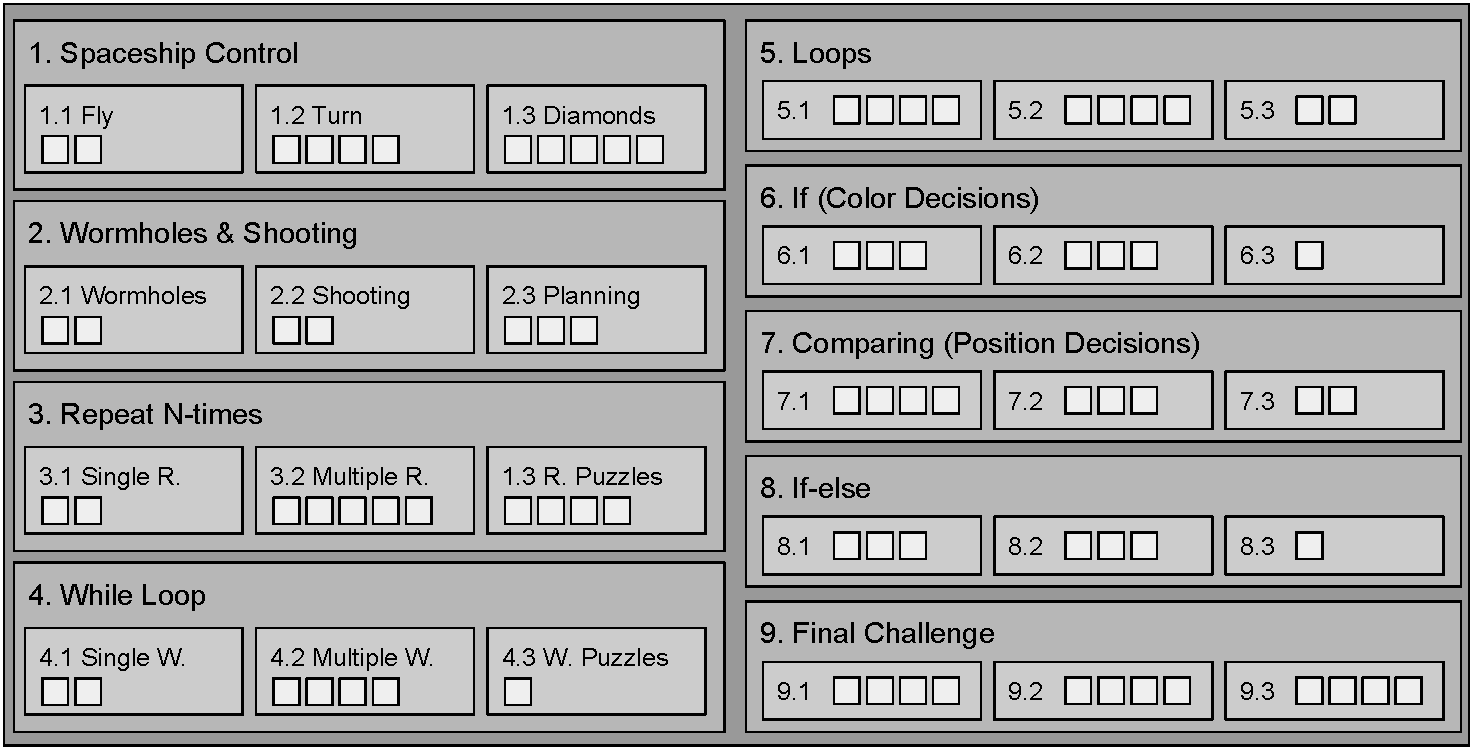
\includegraphics[width=\textwidth,height=.75\textheight,keepaspectratio]{../img/robomission-domain}
\end{figure}
\end{frame}

\begin{frame}{Model studenta}
\begin{figure}
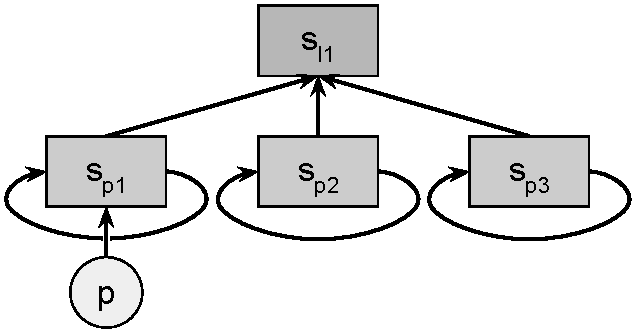
\includegraphics[width=\textwidth,height=.45\textheight,keepaspectratio]{../img/robomission-student-model}
\end{figure}
\end{frame}

\begin{frame}{Doporučování úloh}
% Snaha o optimalni obtiznost -> flow.
% Dekompozice na vyber mise a vyber faze -> nahodna uloha z faze. Mastery learning.
\begin{figure}
\begin{tikzpicture}[font=\sffamily,xscale=5, yscale=5]
\large
\draw [dashed] (0.1,0) -- (1,0.8);
\draw [dashed] (0,0.1) -- (0.8,1);
\draw [thick] (0.0,0.05) -- (0.1,0.05)
           -- (0.1,0.15) -- (0.2,0.15)
           -- (0.2,0.25) -- (0.3,0.25)
           -- (0.3,0.375) -- (0.45,0.375)
           -- (0.45,0.505) -- (0.6,0.505)
           -- (0.6,0.7) -- (0.8,0.7)
           -- (0.8,0.9) -- (1.0,0.9);
\draw [thick, <->] (0,1) node [left] {\emph{obtížnost}} -- (0,0) -- (1,0) node [below right] {\emph{dovednost}};
\node at (0.27,0.82) {frustrace};
%\node at (0.95,0.95) {flow};
\node at (0.7,0.2) {nuda};
\end{tikzpicture}
\end{figure}
\end{frame}

\begin{frame}{Monitoring}
% Google Analytics.
% Monitorovaci nastenka - metriky (napocitavane kazdy noc).
% Tydne updatovany jupyter notebook -- pohodlne rozsirovani.
\begin{figure}
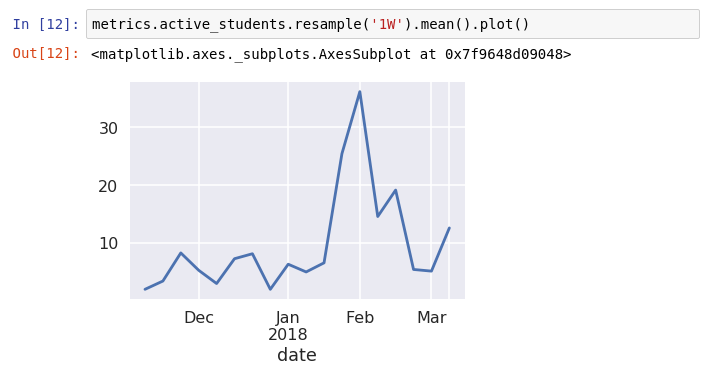
\includegraphics[width=0.62\textwidth]{../img/dashboard-metrics}
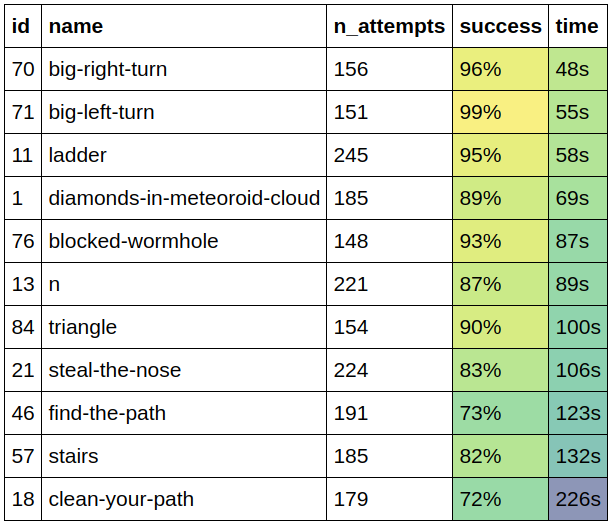
\includegraphics[width=0.37\textwidth]{../img/monitoring-notebook-repeat}
\end{figure}
\end{frame}

\begin{frame}{Počet vyřešených úloh denně}
% Jednoduchý příklad sledované metriky - počet vyřešených úloh denně.
\begin{figure}
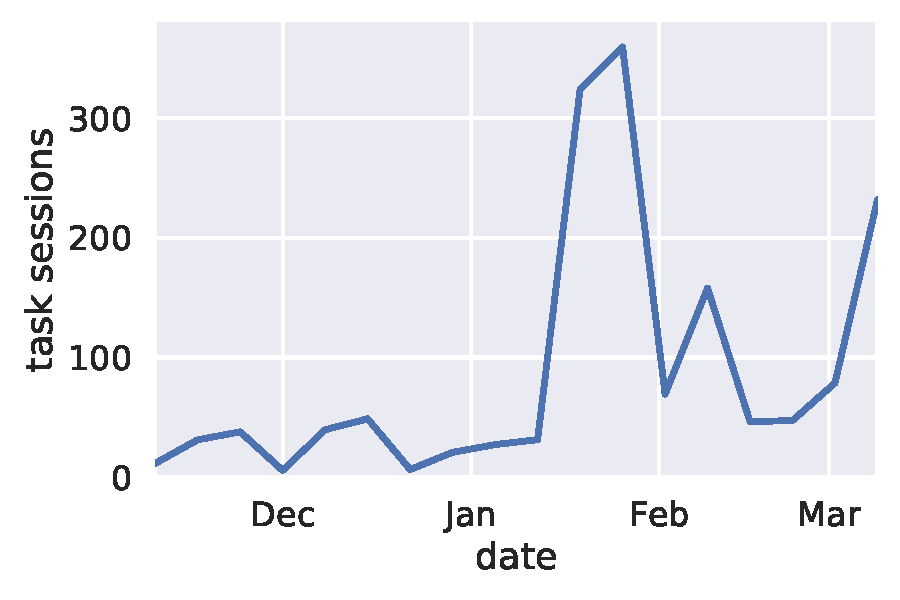
\includegraphics[width=0.7\textwidth]{../img/daily-task-sessions}
\end{figure}
\end{frame}

\begin{frame}{Obtížnost levelů}
% Ukazka analyzy: obtiznost levelu povetsinou roste, ale 7. je tezsi nez 8,
% indikace problemu (jsou tam trikove ulohy na testovani pozice).
% Graf navic ukazuje, ze distribuce casu je zhruba log-normalni.
\begin{figure}
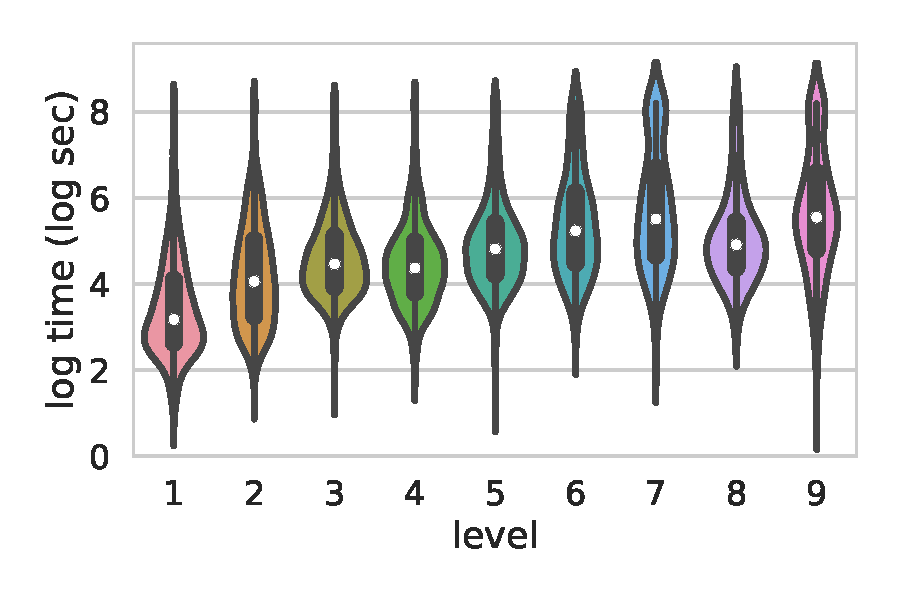
\includegraphics[width=0.8\textwidth]{../img/levels-time}
\end{figure}
\end{frame}

\begin{frame}{Přínosy práce}
\begin{itemize}
\item adaptabilní systém pro výuku programování
      % - navrh a implementace
      % - kombinace strategii pro podporu motivaci i uceni
\item nová výuková hra na mřížce
      % - osvedcene prvky + poutave tema + staly let vpred
      % - blokové programování
\item optimální obtížnost úloh $\rightarrow$ flow
      % - hlavne bonus oproti existujicim systemum
      % - nas pristup k adaptivite, ktery dekomponuje doporucovani uloh
      % na 3 slozky: vyber levelu, vyber faze a mastery learning
\item monitoring, analýza dat
      % monitoring + analyzy -> postupne vylepsovani - nekolik iteraci design loop
      % analyza dat -- 4 mesice pouzivani;
      % -> 2 clanky (navrh adaptability a podobnost polozek), dalsi spousta vyzkumu pred nami
\item testování na školách, použití v soutěžích
\end{itemize}
\end{frame}

%\begin{frame}{Shrnutí}
%\begin{itemize}
%\item adaptabilní systém pro výuku programování
%\item úlohy na mřížce, blokové programování
%\item optimální obtížnost úloh $\rightarrow$ flow
%\item \url{https://robomise.cz}
%%\item kód: \url{github.com/adaptive-learning/robomission}
%\end{itemize}
%\end{frame}

\end{document}
